\documentclass{beamer}
%\usetheme{Ilmenau}
%\usecolortheme{beaver}

\usepackage[slovak,american]{babel}
\usepackage[utf8]{inputenc}
\usepackage{graphicx}
\usepackage{adjustbox}

 \usepackage{xcolor}
 
 \newsavebox\MBox
\newcommand\Cline[2][red]{{\sbox\MBox{$#2$}%
  \rlap{\usebox\MBox}\color{#1}\rule[-2.2\dp\MBox]{\wd\MBox}{1pt}}}

%\usefonttheme{serif}

%\definecolor{UKOrange}{HTML}{ef9424} %
\definecolor{UKOrange}{HTML}{7a2c18} %
\definecolor{UKBrown}{HTML}{a96d5e} %
\definecolor{UKLight}{HTML}{d8b6ab} %
\definecolor{UKDark}{HTML}{7a4f44}
\definecolor{UKDarker}{HTML}{4d312b} 
\definecolor{UKDarkest}{HTML}{2e1e1a}
\definecolor{UKRed}{HTML}{bf1f1c}

\setbeamertemplate{footline}[frame number]{}
\setbeamertemplate{navigation symbols}{}

%\usecolortheme{beaver}
\setbeamertemplate{itemize item}[square]
\setbeamercolor{itemize item}{fg = UKBrown}
\setbeamercolor{itemize subitem}{fg = UKLight}
\setbeamercolor{enumerate item}{fg = UKDark}

\setbeamercolor{footnote}{fg=UKLight}
\setbeamercolor{footnote mark}{fg=UKLight}
\setbeamerfont{footnote}{size=\tiny}
\renewcommand\footnoterule{}

\usetheme{default}
\beamertemplatenavigationsymbolsempty
\setbeamercolor{title}{fg=white, bg=UKBrown}
\setbeamercolor{frametitle}{fg=white, bg=UKBrown}
\setbeamercolor{block title}{bg=UKBrown, fg= white}
\setbeamercolor{block body}{bg =UKLight, fg = UKDarkest}

\setbeamercolor{block title alerted}{bg=UKOrange, fg= white}
\setbeamercolor{block body alerted}{bg =UKLight, fg = UKDarkest}


%\setbeamercolor{section in toc}{fg = UKBrown}
%\setbeamercolor{section in toc}{fg = UKDarkest}

% odstrani gulicky
\renewcommand*{\slideentry}[6]{}

\useoutertheme[subsection=false]{miniframes}
\AtBeginSection[]{\subsection{}}

\setbeamercolor{below lower separation line head}{bg=UKDark}
\addtobeamertemplate{headline}{}{%
  \begin{beamercolorbox}[colsep=0.5pt]{below lower separation line head}
  \end{beamercolorbox}
}
%\setbeamercolor*{mini frame}{fg=white,bg=UKRosy}
\setbeamercolor{section in head/foot}{fg=UKLight, bg=UKDark}

\usepackage{etoolbox}
\makeatletter
\preto{\@verbatim}{\topsep=0pt \partopsep=0pt }
\makeatother

%\setbeamertemplate{itemize/enumerate body begin}{\normalsize}
%\setbeamertemplate{itemize/enumerate subbody begin}{\normalsize}




%\newcommand{\codeblock}[2]{ \begin{block}{#1} \begin{verbatim}#2\end{verbatim}\end{block}}

%\defbeamertemplate*{title page}{customized}[1][]
%{
%  \begin{centering}
%    \begin{beamercolorbox}[sep=8pt,center]{title}
%      \usebeamerfont{title}\inserttitle
%    \end{beamercolorbox}
%  \end{centering}
%  \bigskip
%
%\begin{columns}[onlytextwidth,T]
%
%
%  \column{27mm}
%  \includegraphics[width=27mm]{images/logoFMFI.png}
%  
%  \column{\dimexpr\linewidth-54mm-6mm}
%  \centering
%  \vspace{5mm}  
%  \usebeamerfont{author}\insertauthor\par
%  \vspace{5mm}
%  \usebeamerfont{institute}\insertinstitute\par
%
%  \column{27mm}
%  \includegraphics[width=27mm]{images/logoUK.png}  
%\end{columns}
%\centering
%\vspace{7mm}
%  \usebeamerfont{date}\insertdate\par
%}

\DeclareMathOperator*{\argmin}{arg\,min}
\newcommand{\e}[1]{$\cdot 10^{#1}$}

%\newcommand{\codeblock}[2]{ \begin{block}{#1} \begin{verbatim}#2\end{verbatim}\end{block}}


\title[6. cvičenie]{Advanced Image Processing - Edge Detection}
\author[Kocur]{Ing. Viktor Kocur \\{\small viktor.kocur@fmph.uniba.sk}}
\institute{DAI FMFI UK}
\date{30.10.2019}

\begin{document}
\selectlanguage{slovak}

\begin{frame}
  \titlepage
\end{frame}

\section{Edge Detection}
\subsection{The Process}

\begin{frame}
\frametitle{The Process}
  \begin{block}{Finding edges}
  In case of a continuous functions the edges are found using derivatives. Some methods use the first derivatives while others use the second ones.
  \end{block}

  \begin{center}
  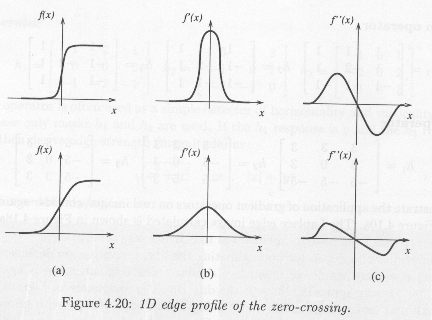
\includegraphics[width=0.6\textwidth]{zero-crossing.png}
  \end{center}
\end{frame}

\begin{frame}
\frametitle{2D discrete case}
  \begin{block}{Discrete case}
  Image is discrete therefore we will utilize differences instead of derivatives. In other words the discrete version of the derivative.
  \end{block}

  \begin{block}{2D}
  The image is 2-dimensional we therefore use partial differences in different directions.
  \end{block}
\end{frame}

\subsection{First derivative}

\begin{frame}
\frametitle{Using the first derivative}
  \begin{block}{Convolution}
  We compute the difference with convolution operation in a similar manner to smoothing.
  \end{block}

  \begin{block}{Exercise}
  Use conv2 and the Prewitt filters to find the edges in the image zatisie.jpg Do not forget to use rgb2gray. Since we have two filters use $h = \sqrt{h_x^2 + h_y^2}$ to obtain combined edges. After the filtration use thresholding to show the edges. 
  \end{block}
 
  \begin{block}{Prewitt filters}
  \begin{center}
  $\begin{matrix}
    1 & 0 & -1 &    & 1 & 1 & 1 \\
    1 & 0 & -1 & a & 0 & 0 & 0 \\
    1 & 0 & -1 &    & -1 & - 1 & -1
  \end{matrix}$
  \end{center}
  \end{block}
\end{frame}

\begin{frame}
\frametitle{Matlab - edge}
  \begin{block}{edge}
  edge(I, method) - returns edge image based on the method. First derivative methods are 'Sobel', 'Prewitt', 'Roberts' and 'Canny'. Second derivative methods are 'log' also known as Marr-Hildreth method.
  \end{block}
 
  \begin{block}{edge}
  edge(I, method, threshold, direction) - It is also possible to specify threshold to use and the direction of the filter.
  \end{block}
\end{frame}

\begin{frame}
\frametitle{Exercise}
  \begin{block}{Exercise}
  Test the edge detection algotihms based on the first derivative.
  \end{block}
    
  \begin{block}{Noise}
  Edge detection can fail with noisy image. Add noise to the image and try to detect edges in the image. Try to perform edge detection after smoothing. Does the result improve?
  \end{block} 
\end{frame}

\begin{frame}
\frametitle{Canny detector}
  \begin{block}{Gauss smoothing}
  Canny detector first smooths the image using the Gaussian filter.
  \end{block}    
  
  \begin{block}{Non-maximum suppression}
  After smoothing a different detector using the first derivative is used. Since simple methods create edges too wide. In each area only the strongest edge is kept. This takes the direction of the edge into consideration.
  \end{block}  
  
  \begin{block}{Weak and strong edge}
  In the end two thresholds are used to divide the remaining edge pixels to two categories: strong and weak edges. Strong edges are kept. From the weak edges only the ones connected to the strong edges are kept.
  \end{block}
\end{frame}

\subsection{Second derivative method}

\begin{frame}
\frametitle{Second derivative method}
  \begin{block}{Second derivative}
  We can find the edge in positions where the second derivative changes sign (zero-crossing).
  \end{block}
    
  \begin{center}
  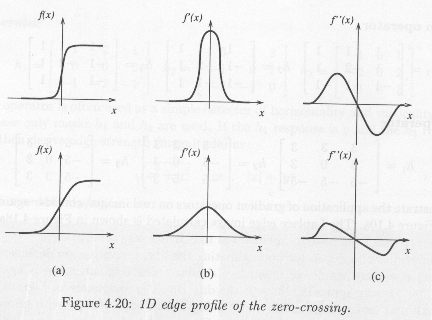
\includegraphics[width=0.6\textwidth]{zero-crossing.png}
  \end{center}
\end{frame}

\begin{frame}
\frametitle{Marr-Hildreth method}
  \begin{block}{LoG}
  To obtain the second derivative the Laplacian of Gaussian filter is used.
  \begin{equation*}
  LoG = -\frac{1}{\pi \sigma^4} \left[ 1 - \frac{x^2 + y^2}{2\sigma^2} \right] e^{-\frac{x^2+y^2}{2\sigma^2}}
  \end{equation*}  
  \end{block}
    
  \begin{center}
  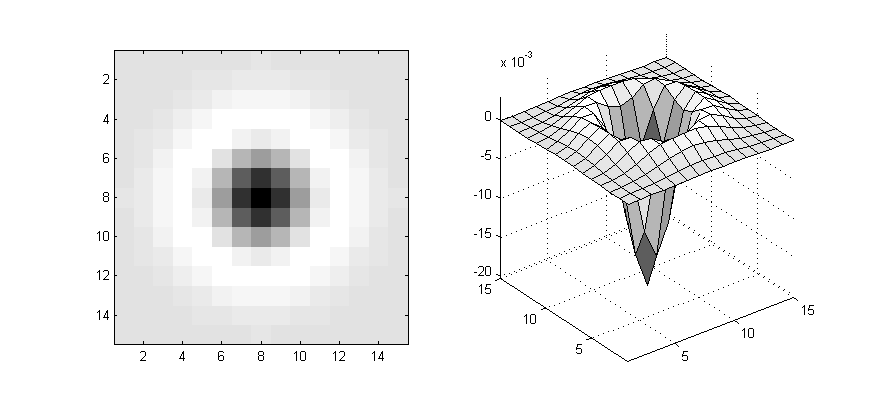
\includegraphics[width=0.8\textwidth]{laplacian_of_gaussian.png}
  \end{center}
\end{frame}

\begin{frame}
\frametitle{Marr-Hildreth method}
  \begin{block}{Zero-Crossings}
  After application of the filter the zero-crossings have to be found.
  \end{block}
  
  \begin{block}{Faster method}
  It is possible to use difference of Gaussians (DoG) instead of LoG.
  \end{block}   
  
  \begin{block}{Exercise}
  Use the Marr-Hildreth method denoted as 'log' to detect edges.
  \end{block}     
\end{frame}


\section{Image sharpening}
\subsection{Unsharp Masking}

\begin{frame}
\frametitle{Unsharp masking} 
\noindent\makebox[\textwidth]{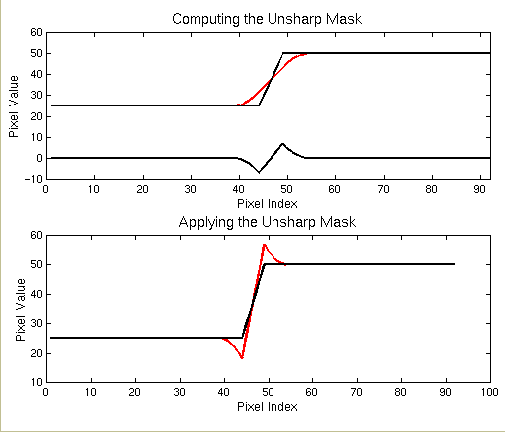
\includegraphics[width=0.9\linewidth]{unsharp.png}}
\end{frame}

\begin{frame}
\frametitle{Unsharp masking} 
  \begin{block}{Sharpening}
    We want to sharpen a blurred image. This task is similar to amplifying the edges.
  \end{block} 
 
  \begin{block}{Unsharp masking - princíp}
    $I_{sharp} = I_{original} + p \cdot \left( I_{original} - I_{smooth} \right)$
  \end{block}
  
  \begin{block}{Úloha}
  Create a function unsharp\_mask(I,p,sigma), which applies unsharp masking with the parameter p with the use of addiive Gaussian noise with the parameter sigma. Apply this on the image blurred.pgm
  \end{block}
\end{frame}

\subsection{Laplace operator}

\begin{frame}
\frametitle{Laplace operator} 
  \begin{block}{Laplace operator - definition}
    $$\Delta f = \nabla \cdot \nabla f = \sum_{i=1}^n \frac{\partial^2 f}{\partial x_i^2} \stackrel{2D}{=} \frac{\partial^2 f}{\partial x^2} + \frac{\partial^2 f}{\partial y^2}$$
  \end{block}
  
  \begin{block}{Convolution kernels in 2D}
  $$\begin{bmatrix}
    1 & 1 & 1 \\
    1 & -8 & 1 \\
    1 & 1 & 1 
   \end{bmatrix}
   or
   \begin{bmatrix}
    0 & 1 & 0 \\
    1 & -4 & 1 \\
    0 & 1 & 0 
   \end{bmatrix}$$
  \end{block}
    
 \begin{block}{Laplace operator in matlab}
 We can generate manually or by using fspecial('laplacian',alpha), where alpha determines how strong is the presence of the diagonal neighbors.
  \end{block}
\end{frame}

\begin{frame}
\frametitle{Image sharpening using the Laplace operator} 
  \begin{block}{Application}    
    $I_{ostr\acute{y}} = I_{origin\acute{a}l} - p \left( L_{jadro} \ast I_{origin\acute{a}l}\right)$
  \end{block}

  \begin{block}{Exercise}
  Load the image blurred.pgm and use Laplace sharpening on it. Use different values of p. Do not forget about data types.
  \end{block}
\end{frame}


\end{document}